% \section{Sistemi Operativi per smartphone: \\ Android e iOS}
\chapter{S.O. per smartphone:\\Android e iOS}
L'applicazione è stata realizzata tramite il framework Flutter (a cui sarà
dedicato l'intero prossimo capitolo), in modo tale da poter sviluppare lo stesso
progetto per i due maggiori sistemi operativi per smartphone: Android di
proprietà di Google e iOS dell'azienda Apple. In questo capitolo si prendono in
considerazione tali sistemi focalizzandosi soprattutto sul funzionamento.

\section{Android}
% \subsection{Android}
Android è un sistema operativo mobile, realizzato per dispositivi mobili
touchscreen, ed è stato sviluppato inizialmente dall'azienda Android Inc., che
nel 2005 è stata acquistata da Google.\\
Una delle caratteristiche più importanti di questo sistema operativo è che
detiene una licenza open source. Questo tipo di licenza consente a
qualsiasi utente di modificare e distribuire liberamente il codice
sorgente, consentendo quindi una continua evoluzione del sistema operativo e una
più semplice diffusione. Considerando i processi, Android riesce a gestirli in
modo da mantenere il consumo energetico al minimo. Quando un’applicazione non è
in uso, il sistema sospende il suo funzionamento ma allo stesso tempo la rende
disponibile per l’uso immediato, così che l’applicazione non contribuisca
al consumo della batteria. Il sistema operativo gestisce le applicazioni archiviate in
memoria, in modo tale che sull'esaurirsi della memoria volatile il sistema inizi
automaticamente a chiudere i processi, partendo da quelli che sono rimasti
inattivi per il periodo di tempo più lungo.

\subsection{Kernel Linux e Architettura}
% \subsubsection{Kernel Linux e Architettura}
Un kernel può essere considerato come un ponte tra hardware e software, e può comunicare con
l’hardware tramite i driver che sono inclusi al suo interno. In questo modo, quando
un’applicazione vuole rispondere a un comando, può inoltrare le istruzioni al
kernel e quest’ultimo può utilizzare i driver dell’hardware che si vuole
controllare per ottenere il comportamento desiderato. In particolare, Android si
appoggia al kernel Linux. Esso fornisce
tutte le funzioni essenziali per il sistema, tra cui la gestione della memoria
primaria e la gestione delle risorse hardware del sistema e delle periferiche.
Il suo incarico quindi è quello di gestire
il tempo processore, le comunicazioni e la memoria, assegnando ogni cosa ai processi in
corso in base alle priorità assegnate. Il kernel Linux è adatto a tutte quelle
tecnologie embedded più rilevanti, e quindi ha avuto molto successo nel campo
delle tecnologie portatili.
Esso è inoltre utilizzato dal sistema operativo Android, sebbene Google abbia
introdotto qualche variazione. Una di queste è la funzionalità di gestione
del risparmio, chiamata \textit{wakelocks}, che impedisce al telefono di lavorare a
basso consumo. Nel kernel Linux non c’è un’implementazione completa della
Libreria Standard del linguaggio C++ (STL), dato che le applicazioni Android si
basano sul linguaggio di programmazione Java. Da questo segue che per svolgere
la propria funzione tutte le chiamate a
sistema fatte in C/C++ devono richiamare la Java Virtual Machine. Oltre al
kernel Linux, Android è formato anche da  middleware, Librerie e API scritte in
C/C++ (fig. \ref{kernel}). Le
ultime versioni di Android usano ART Virtual Machine, mentre nelle vecchie versioni
veniva utilizzata la Dalvik Virtual Machine (entrambe considerate nel prossimo
paragrafo).
\begin{figure}
    \centering
    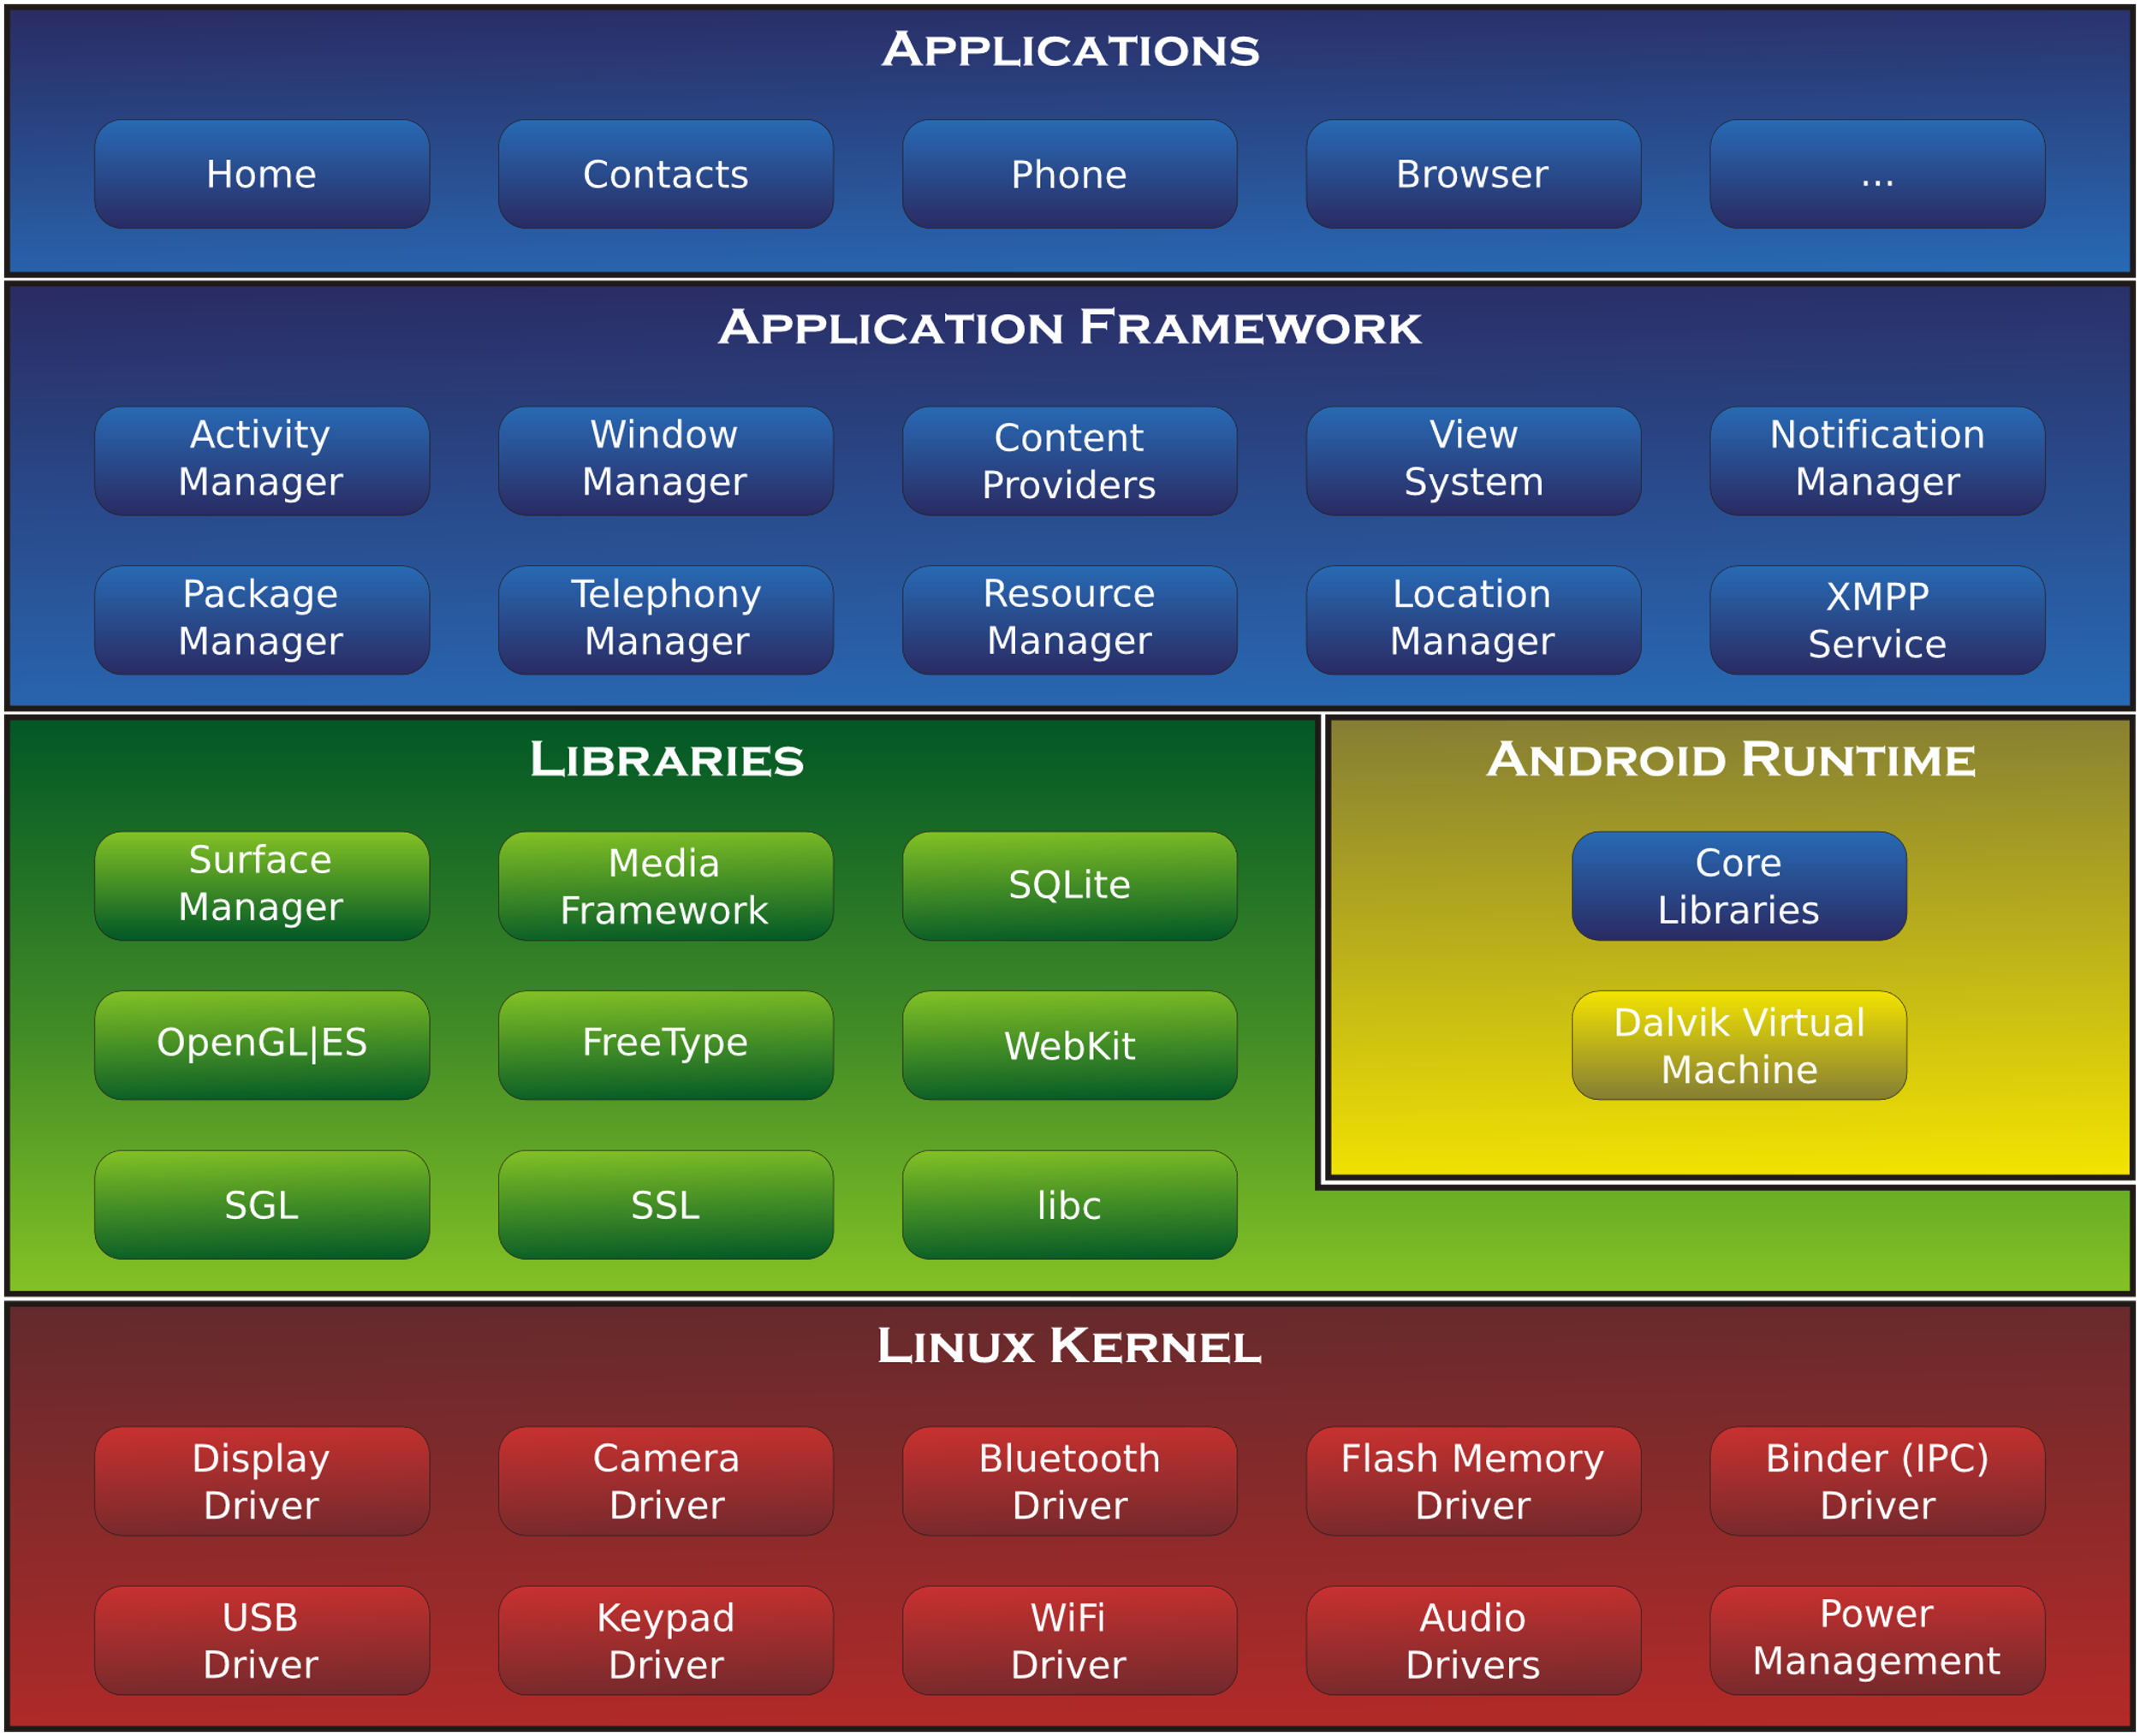
\includegraphics[width=9.5cm]{kernel.png}
    \caption{Struttura del sistema operativo Android e del kernel Linux}
    \label{kernel}
\end{figure}

\subsection{ART Virtual Machine e Dalvik Virtual Machine}
% \subsubsection{ART Virtual Machine e Dalvik Virtual Machine}
La VM, Virtual Machine, è in Android il software all’interno del
quale vengono eseguite le applicazioni. Le applicazioni Android vengono scritte in
linguaggio Java, il quale viene poi compilato in Bytecode
(intermedio tra il linguaggio macchina e il linguaggio di
programmazione che permette che il codice possa essere eseguito su macchine
diverse con hardware diversi), compilato infine
dalla Virtual Machine. Inizialmente in Android veniva utilizzata la Dalvik VM,
che a partire dalla versione 4.4 KitKat di Android, è stata sostituita dalla ART
VM.
La VM Dalvik è basata su tecnologia \textit{just-in-time}: ogni applicazione viene
compilata solo in parte dal programmatore e sarà poi di volta in volta dovere
della Dalvik VM eseguire il codice e compilarlo in linguaggio macchina in tempo
reale. Questo ovviamente grava sulle prestazioni.
La ART VM (Android Run Time) invece è basata su tecnologia \textit{ahead-of-time} che esegue l'intera
compilazione del codice durante l'installazione dell'applicazione e non durante
l'esecuzione stessa del software. Questo permette di avere un vantaggio in
termine di prestazioni, anche se incide sul tempo di installazione delle
applicazioni.

\subsection{Sviluppo applicazioni in Android}
% \subsubsection{Sviluppo applicazioni in Android}
In aiuto ai programmatori per la scrittura di applicazioni Android esiste un
kit di sviluppo software  chiamato SDK. L’SDK  comprende un numeroso set di
strumenti di sviluppo, tra cui: librerie software, debugger, documentazione e
codice d’esempio. Esistono poi diversi ambienti per lo sviluppo, tra questi si
ricordano Visual Studio Code, Atom, Eclipse e Android Studio. Quest'ultimo è considerato l'IDE
primario per lo sviluppo di applicazioni, in quanto presenta notevoli agevolazioni.
I progetti Android sono costituiti da parti dinamiche scritte in Java e
parti statiche scritte in XML. L’SDK permette  di eseguire le applicazioni sia
in emulazione, sia su un dispositivo vero e proprio. Per descrivere
l’applicazione allo smartphone che si vuole utilizzare, si fa ricorso al file
Manifest.xml, questo elenca la lista delle necessità del software per poter
funzionare in modo adeguato. Per motivi di sicurezza, per evitare che
applicazioni di terze parti abbiano i permessi per poter accedere a informazioni
private all’interno del
telefono, bisogna controllare attentamente il contenuto del Manifest, e non
installare il software in caso richieda risorse non coerenti con lo scopo
dichiarato dell’applicazione. Una volta scritta e concluso il progetto, il
codice java e il codice XML vengono compilati generando un file con estensione
.apk (l’eseguibile delle applicazioni Android). Esso contiene il bytecode che verrà
eseguito dalla Virtual Machine. Le applicazioni Android sono pilotate
dagli eventi (Event Driven), causati da hardware o da altri
componenti. Il programmatore quindi sviluppa per ogni hardware routine
indipendenti, permettendo al sistema operativo di rinunciare al caricamento di
componenti che non si andranno a utilizzare, facendo uso solo di quelli che sono
strettamente necessari. \\
Quando si avvia per la prima volta un dispositivo Android, si può notare come su
tale sistema siano già presenti
applicazioni di terze parti, che possono essere utilizzate fin da subito
dagli utenti. Quando si vuole utilizzare un'applicazione non ancora presente sul
proprio smartphone bisogna scaricare e installare il file apk dell’applicazione
dal Google Play Store. Quest’ultimo è il principale "negozio" di
applicazioni installato su dispositivi Android, e consente agli utenti di
scaricare e aggiornare le applicazioni pubblicate da Google o sviluppatori di
terze parti. Esistono infine anche un certo numero di store di app di terze
parti, che forniscono servizi che non possono essere offerti dallo store
ufficiale a causa di violazioni di particolari norme.

\section{iOS}
% \subsection{iOS}
Il sistema operativo creato da Apple è esclusivo dei propri device, in quanto
solo gli iPhone presentano questo software poichè l'azienda, a differenza di
Android, non concede licenze per l’installazione di iOS su hardware diverso da quello
proprietario. Nonostante questo è però il secondo
sistema operativo mobile più popolare al mondo. \\
Per lo sviluppo di queste applicazioni viene messo a disposizione un SDK apposito,
disponibile unicamente per PC Mac. L’SDK contiene diversi strumenti che
consentono ai programmatori di utilizzare le varie funzioni e servizi dei
dispositivi iOS. Il Software Development Kit, in coppia con XCode, assiste gli
sviluppatori a scrivere
applicazioni per Apple utilizzando linguaggi di programmazione ufficialmente
supportati (Swift
e Objective-C). Xcode è un ambiente di sviluppo per macOS adibito allo sviluppo
di software in grado di essere esguito sui dispositivi dell'azienda di
Cupertino. La suite Xcode include la maggior parte
della documentazione per sviluppatori di Apple e con un Interface Builder integrato,
(applicazione facile e intuitiva utilizzata per costruire interfacce utente
grafiche) Al suo interno è anche presente un simulatore in grado di creare un
iPhone virtuale all'interno del proprio Mac su cui poi testare le applicazioni
sviluppate.
\subsection{Architettura}
% \subsubsection{Architettura}
Le app interagiscono con l’hardware attraverso una serie di interfacce di
sistema. Queste interfacce semplificano la scrittura di applicazioni per i
dispositivi Apple. I livelli inferiori forniscono servizi di base a cui tutte le
applicazioni fanno affidamento, quelli superiori invece forniscono servizi
per avere una grafica di alto livello. iOS usa kernel XNU (\textit{X is Not
Unix}) ed è caratterizzato da
4 livelli di astrazione: il Core OS Layer, il Core Services Layer, il Media layer e
il Cocoa Touch Layer (fig. \ref{ios1}). Ogni livello ha una serie di framework
utilizzabili dagli sviluppatori. 
\begin{figure}[!h]
    \centering
    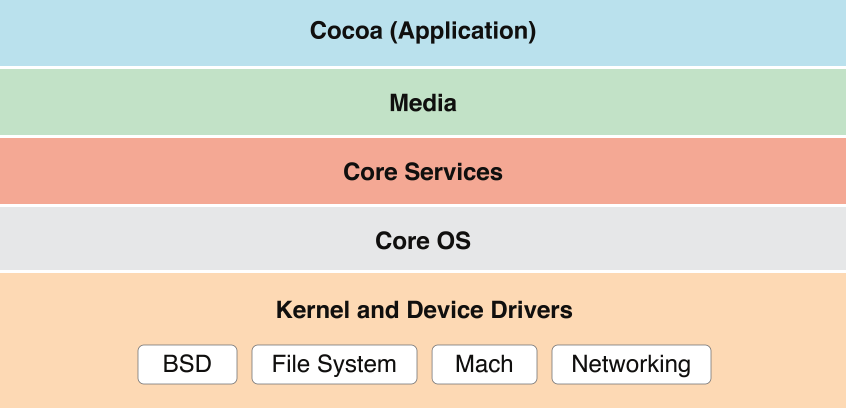
\includegraphics[width=9cm]{ios1.png}
    \caption{Struttura del sistema operativo iOS}
    \label{ios1}
\end{figure}

Il livello più basso di iOS è costituito dal kernel di cui si parlerà nel
prossimo paragrafo. Al di sopra del kernel, si ha il Core OS,
responsabile della gestione della memoria, delle attività del file system, della
rete e delle attività del sistema operativo ed interagisce anche con l’hardware.
Al livello successivo è presente il Core Services, il quale fornisce servizi Peer-to-Peer,
archiviazione su iCloud, protezione dati, supporto per condivisione di file, Grand
Central Dispatch, SQLite, supporto XML e gestisce anche gli acquisti in app. Successivamente
si ha il Media Layer, che fornisce al sistema operativo funzionalità audio, video
e animazioni. L’ultimo livello, il Cocoa Touch, contine framework molto importanti
che definiscono l’aspetto dell’app. Esso fornisce anche l'infrastruttura di base delle
applicazioni e supporto per tecnologie importanti come multitasking, touch,
notifiche push e per altri aspetti di alto livello.

\subsection{Kernel XNU}
% \subsubsection{Kernel XNU}
Il kernel XNU, come detto precedentemente, fa da mediatore tra il software
e l’hardware, ed è il primo programma ad essere caricato in memoria
all’accensione del dispositivo. XNU è utilizzato nel sistema operativo open source
Darwin, ed Apple lo usa come base per il proprio software. Esso è inoltre
ibrido, poiché formato da due tipologie di kernel: il microKernel Mach e il
Kernel BSD (fig. \ref{ios2}).
Inoltre XNU è modulare, ovvero è possibile utilizzare moduli aggiuntivi
attivabili e disattivabili durante il funzionamento. \\
Il primo componente, il vero e proprio cuore di XNU, è Mach, microkernel che gestisce le
responsabilità elementari del sistema operativo: scambio di messaggi tra
processi, pianificazione delle attività, gestione della memoria virtuale ed
elaborazione dei thread. Il secondo componente è il kernel BSD, che fornisce un
livello di astrazione superiore e permette l’accesso ai dispositivi e al file
system. L’ultimo componente è il framework I/O Kit, completamente indipendente
dal kernel e consente agli sviluppatori di creare rapidamente driver per i
dispositivi. \\
\begin{figure}[!h]
    \centering
    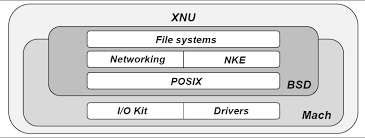
\includegraphics[width=11cm]{ios2.png}
    \caption{I diversi livelli e sezioni del kernel XNU}
    \label{ios2}
\end{figure}


